\section{Sequence to Sequence}
\label{chap:Sequence to Sequence}

  %%%%%%%%%%%%%%%%%%%%%%%%%%%%
  % SUBSECTION               %
  %%%%%%%%%%%%%%%%%%%%%%%%%%%%
\subsection{Introduction}
Deep Neural Networks (DNNs) are extremely powerful machine learning models that achieve excellent performance on difficult problems such as machine translation, speech recognition, and text automated QA. DNNs are powerful because they can perform arbitrary parallel computation
for a modest number of steps. Large
DNNs can be trained with supervised backpropagation whenever the labeled training set has enough information to specify the network’s parameters according to \textit{Sequence to Sequence Learning
with Neural Networks} paper. \cite{web015}\\
Seq2seq models have enjoyed great success in a variety of tasks.
It is a relatively new paradigm,
with its first published usage in 2014 for English-French translation at a high level.
\subsection{Neural Machine Translation with Seq2Seq} 
There’s a whole
class of NLP tasks that rely on sequential output, or outputs that are
sequences of potentially varying length. For example,\\
• Translation: taking a sentence in one language as input and outputting
the same sentence in another language.\\
• Conversation: taking a statement or question as input and responding
to it.\\
• Summarization: taking a large body of text as input and outputting
a summary of it.
\\Neural Machine Translation (NMT) which was the very first testbed for seq2seq models with wild success \cite{web016}. A seq2seq model is an end-to-end model made up of two recurrent neural networks: an encoder, which takes the model’s input sequence as input and
encodes it into a fixed-size "context vector", and a decoder, which uses the context vector from above as a "seed"
from which to generate an output sequence. For this reason, Seq2Seq models are often referred to as "encoder-decoder
models." An encoder converts a source sentence into a "Meaning" or "Thought" vector which is passed through a decoder to produce a translation.\\
  \begin{figure}[H]%
    \center%
    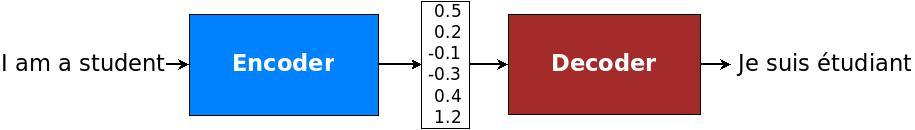
\includegraphics[width=\textwidth]{images/amir/encdec.jpg}%
     % you need to add the caption for the list of figures
    \caption[Encoder part of seq2seq]{encoder-decoder as seq2seq}\label{fig:encdec}%
  \end{figure}
  Back in the old days, traditional phrase-based translation systems performed their task by breaking up source sentences into multiple chunks and then translated them phrase-by-phrase. This led to disfluency in the translation outputs and was not quite like how we, humans, translate. We read the entire source sentence, understand its meaning, and then produce a translation. Neural Machine Translation (NMT) mimics that!\\
  NMT addresses the local translation problem in the traditional phrase-based approach; it can capture long-range dependencies in languages, e.g., gender agreements; syntax structures; etc., and produce much more fluent translations as demonstrated by \textit{Google Neural Machine Translation} systems \cite{web017}.\\
  At a high level, the NMT model consists of two recurrent neural networks: the encoder RNN simply consumes the input source words without making any prediction; the decoder, on the other hand, processes the target sentence while predicting the next words.
   \begin{figure}[H]%
    \center%
    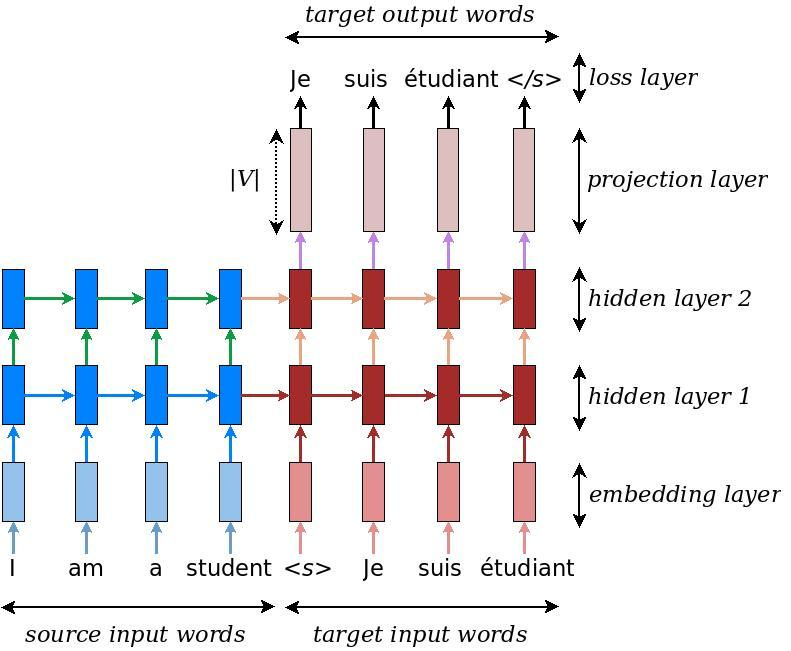
\includegraphics[width=.6\textwidth]{images/amir/seq2seq.jpg}%
     % you need to add the caption for the list of figures
    \caption[seq2seq architecture]{ seq2seq-NMT architecture
    }\label{fig:seq2seq}%
  \end{figure}
  \subsubsection{Seq2Seq architecture - Encoder}
  The encoder network’s job is to read the input sequence to our
Seq2Seq model and generate a fixed-dimensional context vector C
for the sequence. To do so, the encoder will use a recurrent neural
network cell – like GRU - to read the input tokens one at a time. The final hidden state of the cell will then become C as our "Thought" vector.\\
 However,
because it’s so difficult to compress an arbitrary-length sequence into
a single fixed-size vector (especially for difficult tasks like translation),
the encoder will usually consist of stacked GRUs: a series of
GRU "layers" where each layer’s outputs are the input sequence to
the next layer. The final layer’s GRU hidden state will be used as C.
 \begin{figure}[H]%
    \center%
    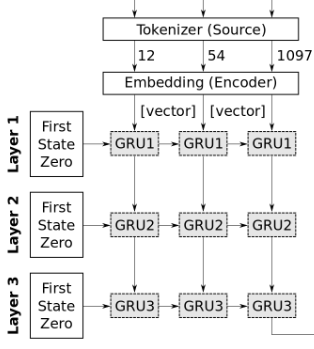
\includegraphics[width=.4\textwidth]{images/amir/enc.png}%
     % you need to add the caption for the list of figures
    \caption[Encoder Details]{ a look inside Encoder architecture \cite{web018}
    }\label{fig:encoder}%
  \end{figure}
Seq2Seq encoders will often do something strange: they will process
the input sequence in reverse. This is actually done on purpose.
The idea is that, by doing this, the last thing that the encoder sees
will (roughly) corresponds to the first thing that the model outputs;
this makes it easier for the decoder to "get started" on the output,
which makes then gives the decoder an easier time generating a
proper output sentence. In the context of translation, we’re allowing
the network to translate the first few words of the input as soon as it sees them; once it has the first few words translated correctly, it’s
much easier to go on to construct a correct sentence than it is to do
so from scratch. \\
\textit{Note that the input
tokens are read in reverse. Note that the
network is unrolled; each column is a
timestep and each row is a single layer,
so that horizontal arrows correspond
to hidden states and vertical arrows are
GRU inputs/outputs.}
\subsubsection{Seq2Seq architecture - Decoder}
The decoder is also an GRU network, but its usage is a little more complex than the encoder network. Essentially, we’d like to use it as a language model that’s "aware" of the words that it’s generated
so far and of the input. To that end, we’ll keep the "stacked" GRU
architecture from the encoder, but we’ll initialize the hidden state of
our first layer with the context vector from above; the decoder will
literally use the context of the input to generate an output.
\begin{figure}[H]%
    \center%
    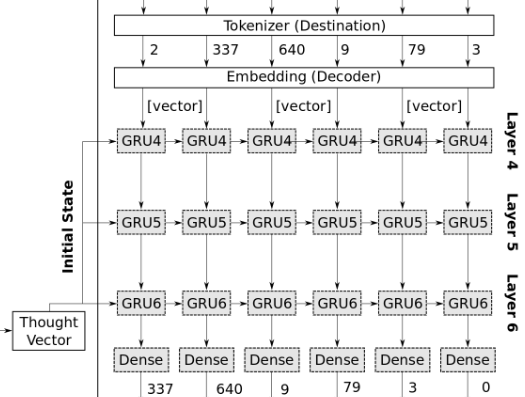
\includegraphics[width=.6\textwidth]{images/amir/dec.png}%
     % you need to add the caption for the list of figures
    \caption[Decoder Details]{ a look inside Decoder architecture \cite{web018}
    }\label{fig:decoder}%
  \end{figure}
Once the decoder is set up with its context, we’ll pass in a special
token to signify the start of output generation; in literature, this is
usually an (EOS) token appended to the end of the input (there’s
also one at the end of the output).
Then, we’ll run all three layers of
GRU, one after the other, following up with a softmax on the final
layer’s output to generate the first output word.\\
Once we have the output sequence, we use the same learning strategy
as usual. We define a loss, the cross entropy on the prediction
sequence, and we minimize it with a gradient descent algorithm and
back-propagation. Both the encoder and decoder are trained at the
same time, so that they both learn the same context vector representation.
\subsection{Using Attention Mechanism}
When you hear the sentence "the ball is on the field," you don’t assign
the same importance to all 6 words. You primarily take note of
the words "ball," "on," and "field," since those are the words that are
most "important" to you.  Similarly, the flaw
in using the final RNN hidden state as the single "context vector" for
seq2seq models; it seems somewhat unreasonable to assume that we can encode all information about a potentially very long sentence into a single vector and then have the decoder produce a good translation based on only that.\\ Often, different parts of an input have different levels of significance. Moreover, different parts of the output
may even consider different parts of the input "important."Attention mechanisms make use of this observation by providing
the decoder network with a look at the entire input sequence at every
decoding step; the decoder can then decide what input words are
important at any point in time.\\
\begin{figure}[H]%
    \center%
    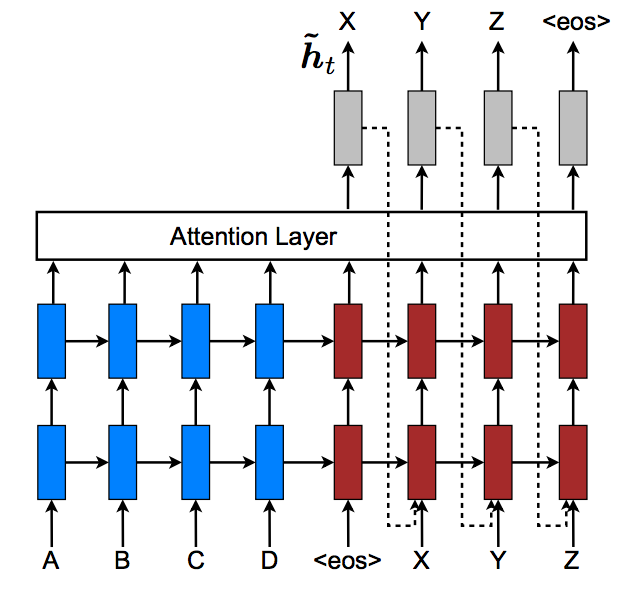
\includegraphics[width=.5\textwidth]{images/amir/Feeding-Hidden-State-as-Input-to-Decoder.png}%
     % you need to add the caption for the list of figures
    \caption[Attention Layer]{using  attention as a layer
    }\label{fig:attention}%
  \end{figure}
RNNs are known to have problems dealing with such long-range dependencies. In theory, architectures like LSTMs or GRUs should be able to deal with this, but in practice long-range dependencies are still problematic.\\
For example, researchers have found that reversing the source sequence (feeding it backwards into the encoder) produces significantly better results because it shortens the path from the decoder to the relevant parts of the encoder. Similarly, feeding an input sequence twice also seems to help a network to better memorize things.\\
With an attention mechanism we no longer try encode the full source sentence into a fixed-length vector. Rather, we allow the decoder to “attend” to different parts of the source sentence at each step of the output generation. Importantly, we let the model learn what to attend to based on the input sentence and what it has produced so far.\cite{web019}
\subsubsection{Performance, Areas and Cost}
That attention overcomes the limitation in the encode-decoder architecture by allowing the network to learn where to pay attention to the input for each item in the output sequence. That the encoder-decoder architecture for recurrent neural networks uses a fixed-length internal representation that imposes a constraint that limits learning very long sequences. So using attention gives a great performance over long sentences 50-70 words.\\ 
\begin{figure}[H]%
    \center%
    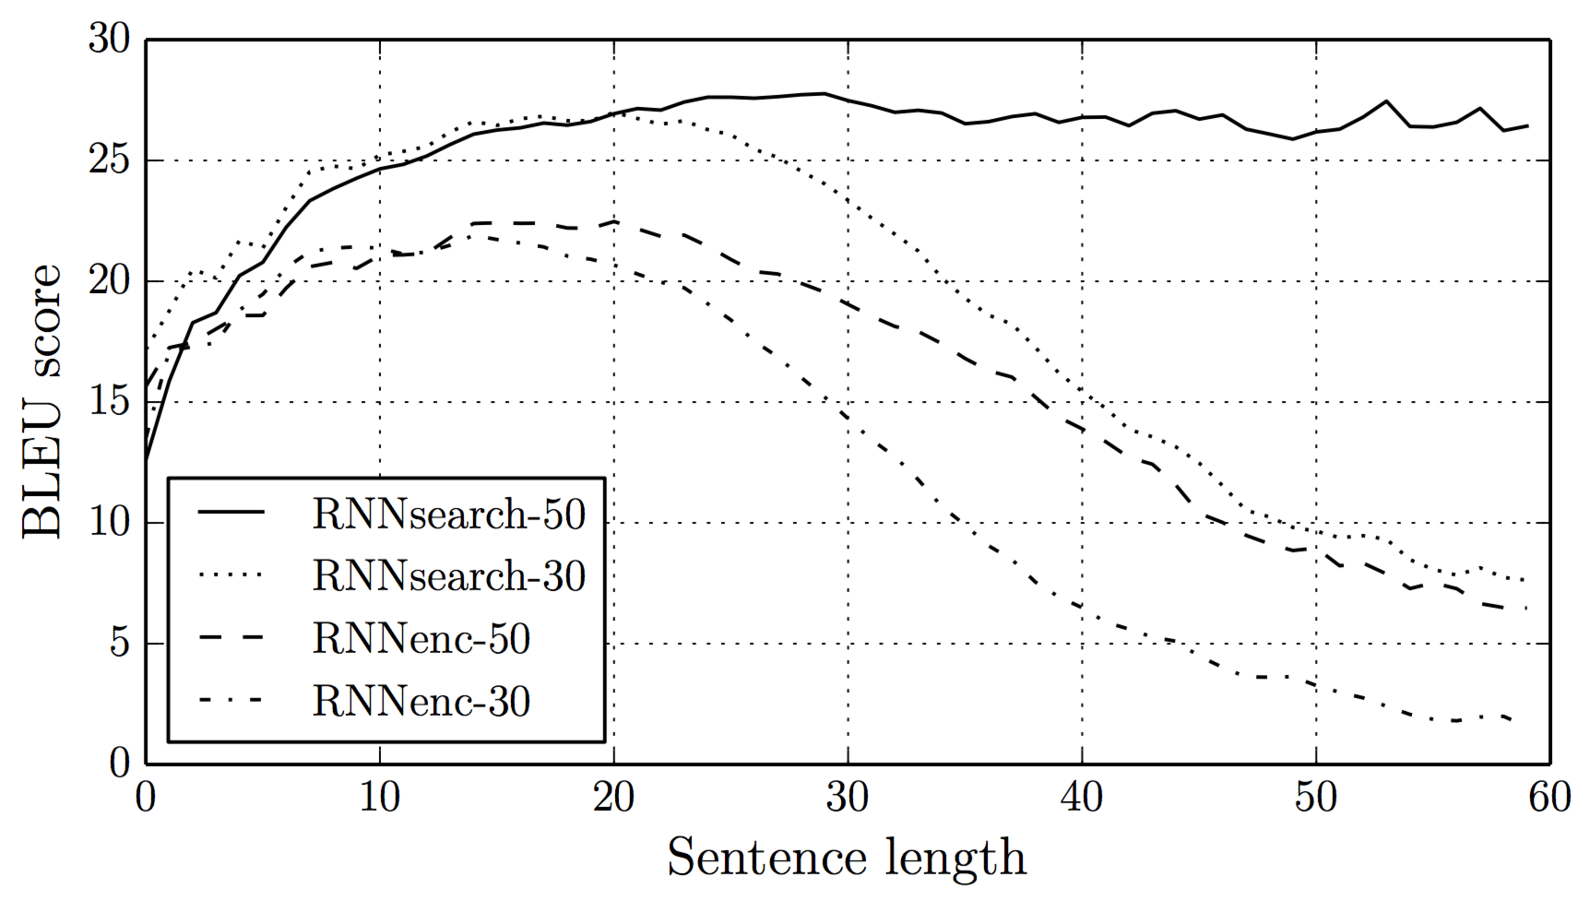
\includegraphics[width=\textwidth]{images/amir/bahdanau_attn.png}%
     % you need to add the caption for the list of figures
    \caption[Attention Performance]{  attention performance over 30 words is clear
    }\label{fig:attention performance}%
  \end{figure}
Because its high performance it is used in Translation and also used fields like Text Summarization, automated QA, Speech Recognition, Entailment, and Image Descriptions.\cite{web020}\\\\
If you have a 50-word input sequence and generate a 50-word output sequence that would be 2500 attention values. That’s not too bad, but if you do character-level computations and deal with sequences consisting of hundreds of tokens the above attention mechanisms can become prohibitively expensive. We’re essentially looking at everything in detail before deciding what to focus on. Still, that hasn’t stopped attention mechanisms from becoming quite popular and performing well on many tasks.\\
An alternative approach to attention is to use Reinforcement Learning to predict an approximate location to focus to. That sounds a lot more like human attention, and that’s what’s done in Recurrent Models of Visual Attention.